\documentclass[10pt,letterpaper,subeqn]{beamer}
\setbeamertemplate{navigation symbols}{}
\usefonttheme{serif}
\usecolortheme{seahorse}


\usepackage[english]{babel}
\selectlanguage{english}
\usepackage{bm}
\usepackage{booktabs}
\usepackage{color}
\usepackage[update,prepend]{epstopdf}
\usepackage{framed}
\usepackage{fleqn}
\usepackage{graphics}
\usepackage{hyperref}
\usepackage[utf8]{inputenc}
\usepackage{setspace}
\usepackage{textcomp}
\usepackage{wrapfig}
\usepackage{multirow}
\usepackage{caption}
\usepackage{subcaption}
\usepackage{subfloat}
\usepackage{hyperref}
\setbeamertemplate{caption}[numbered]
\usepackage{wrapfig}
\usepackage{tikz}

\definecolor{cadmiumgreen}{rgb}{0.0, 0.42, 0.24}
\usetikzlibrary{trees}
\usetikzlibrary{decorations.markings}

%================================================================================
%== TITLE, NAMES, DATE
%================================================================================
\title[Women's Health and Gender Inequality]{Maternal Mortality and Female Life 
Expectancy: The Importance of Gender Inequality} 

 \author[Bhalotra et al.]{Sonia Bhalotra (Essex)
    \and Damian Clarke (Santiago) \\ \vspace{1mm}
    \and Joseph Gomes (Navarra)
    \and Atheen Venkataramani (Mass Gen)}


\date{August 2016}
%********************************************************************************
\begin{document}

\begin{frame}
\titlepage
\end{frame}
%********************************************************************************



\section{Introduction}
\begin{frame}[label=intro]
\frametitle{Importance of historical institutions}
\begin{itemize}
  \setlength{\itemsep}{10pt}
	\item Historical institutions cast long shadows which can explain heterogeneities in contemporary socio-economic outcomes (Acemoglu et al., 2001; Nunn and Wantchekon, 2011).
	\item Not surprisingly history also plays a role in explaining how gender related preferences are formed, contemporary prioritization of women, and variations in women's well being.
	\begin{itemize}
		\item Alesina et al., (2013)- Plough use and the origins of gender roles 
		\item Gay et al., (2013) - The origins of gender roles due to language grammatical structure 
		\item Nunn (2012) - The role of missionaries in explaining female literacy in Africa.
	\end{itemize}
	\item We particularly focus on health outcomes - Maternal Mortality
	\item We first argue that women are a low public policy priority and then ask
	\begin{itemize}
		\item To what extent can this be addressed by manipulating contemporary institutional structures? 
		\item Can the heterogeneity be traced back to deep seated preferences?
	\end{itemize}
\end{itemize}
\end{frame}


\begin{frame}
\frametitle{Women are a low public policy priority.}
\begin{itemize}
  \setlength{\itemsep}{20pt}
	\item MMR decline slower than other infectious diseases.
	\item Infant mortality decline started much earlier and progressed more rapidly 
        than maternal mortality decline.
	\item Infant mortality decline has benefited from massive improvements in 
        control of infectious disease. 
	\item Historically, the same improvements led to maternal mortality declines, 
        consistent with 40-50\% of maternal deaths being the result of post-partum
        puerperal sepsis (an infection).
  \item Our hypothesis: the sluggishness of MMR decline is a function of gender 
        prejudice, (in Med/Public Health: \hyperlink{Yentl}{\textcolor{blue}
        {The Yentl Syndrome}}).
\end{itemize}
\end{frame}


\begin{frame}
\frametitle{Key Questions}
Does giving women voice/decision making capacity in public policy/politics change things? 
\vspace{4.5mm}
\begin{enumerate}
  \setlength{\itemsep}{9.5pt}
	\item Historical reforms (suffrage, sulfonamides) and state-varying MMR reductions.
  \item Contemporary reforms - Quotas and women's representation in parliament.
\end{enumerate}
\vspace{5mm}
Gender prejudice in societies has strong (lethal) implications on women-specific 
health outcomes.  We test this in a number of ways:
\vspace{4.5mm}
\begin{enumerate}
  \setlength{\itemsep}{9.5pt}
  \item Time series and cross-sectional variation in gender inequality and female
        health world-wide
  \item Historical intra-country and cross-country gender prejudice determinants
  \item Examining placebo (gender-neutral) diseases using the same specifications
\end{enumerate}
\end{frame}


\begin{frame}
\frametitle{Related Literature}
\begin{itemize}
\setlength{\itemsep}{20pt}
	\item Literature on missing women
	\begin{itemize}
	\setlength{\itemsep}{10pt}
		\item Sen 1981, 1990, 2003 highlights the deficit of girls age 0-5 particularly in India.\\ \\
		\begin{center}
		\textbf{``More Than 100 Million Women Are Missing"}
		\end{center}
		\item Anderson and Ray 2010, 2012 highlight missing women across the [disease and] age distribution.
		\item They are agnostic about prejudice driving excess mortality amongst women.
		\item We present the first attempt to focus on maternal mortality decline and assess the role of ``cultural factors" conditional upon income (Jayachandran 2014 discusses this in more general terms).
	\end{itemize}
\end{itemize}
\end{frame}


\frame{
\frametitle{Wider Angle: Life Expectancy}
\begin{itemize}
\setlength{\itemsep}{20pt}
	\item In early 20th century America, maternal mortality was the $2^{nd}$ largest cause of death for women of reproductive age, after TB (which affected men equally): Alabanesi \& Olivetti (2009). 
		\vspace{3mm}
		\begin{itemize}
		\setlength{\itemsep}{12pt}
		\item Similar magnitude in poor countries today although also CVD, injuries in India and HIV/AIDS in Africa.
		\end{itemize}
	\item MMR contributes to female life expectancy.
	\vspace{3mm}
		\begin{itemize}
		\setlength{\itemsep}{12pt}
		\item MMR declined by around 30\% in the late 1930s in America, raising the female-male LE differential at age 20 from 1.5 years in 1920 to 6 years in 1960. 
		\item In the OECD the average female advantage in life expectancy during 1960-2011 was 6 years. 
		\item In SS-Africa it is 2-3 years and in S-Asia it is close to zero.
\end{itemize}
\end{itemize}
}

\frame{
\frametitle{MMR: Brazil vs. India - A contrast}
	\begin{itemize}
	\setlength{\itemsep}{20pt}
		\item India: MMR was 390 in 100,000 and women's life expectancy advantage was 0.59 years in 2000. 
		\item Contrast with Brazil: MMR of 84 and women had a LE advantage of 6.1 years.
		\item Brazil adopted the Right to Health and implemented Universal Health Coverage and an emphasis on women's health ahead of other poor countries.
	\end{itemize}
}

%\frame{
%\frametitle{MMR and Excess female mortality}
%\begin{table}[htbp]\centering
%\footnotesize
%\def\sym#1{\ifmmode^{#1}\else\(^{#1}\)\fi}
%\caption{Mortality in the Reproductive ages (15-49)}
%\begin{tabular}{l*{3}{c}}
%\hline\hline
            %&\multicolumn{1}{c}{(1)}&\multicolumn{1}{c}{(2)}&\multicolumn{1}{c}{(3)}\\
            %&\multicolumn{1}{c}{Male}&\multicolumn{1}{c}{Female}&\multicolumn{1}{c}{Ratio (F/M)}\\
%\hline
%Log of MMR        & 0.0326         & 0.0767\sym{**} & 0.0442\sym{**} \\
            %&(0.0373)         &(0.0386)         &  (0.0181)         \\
%[1em]
%Log of GDP      & -0.0877\sym{***}& -0.111\sym{***}&  -0.0229         \\
            %& (0.0320)         & (0.0376)         & (0.0142)         \\
%\hline
%\(N\)       &               697 &         697         &  697         \\
%r2          &           0.0982   &       0.147         &  0.0678         \\
%\hline\hline
%\multicolumn{4}{l}{\footnotesize Standard errors in parentheses. }\\
%\multicolumn{4}{l}{\footnotesize All specifications have country and year FE.}\\
%\end{tabular}
%\end{table}
%}
%


\begin{frame}
\frametitle{Implications for Other Outcomes}
MMR decline not only contributes to improving female life expectancy and child outcomes but also other outcomes.
\vspace{3mm}
\begin{itemize}
\setlength{\itemsep}{20pt}
	\item MMR decline raises
		\vspace{1.5mm}
		\begin{itemize}
		\setlength{\itemsep}{12pt}
			\item women's labour force participation (Alabanesi \& Olivetti 2009) 
			\item women's education (Alabanesi \& Olivetti (2014), Jayachandran \& Lleras-Muney 2008).
		\end{itemize}
		\item Gender equality in general and MMR decline in particular have been linked to economic growth (Lagerlof 2003, Amiri and Gerdtham 2013, Kirigia et al 2006).
		\item MMR decline tends to raise fertility, although concurrent IMR decline tends to lower fertility (Bhalotra \& Venkataramani 2014).
\end{itemize}
\end{frame}


\frame{
\frametitle{Hypothesis}
\begin{itemize}
\setlength{\itemsep}{20pt}
		\item Mechansim?
		\vspace{3mm}
	\begin{itemize}
	\setlength{\itemsep}{15pt}
		\item Son preference - high \textit{fertility} - higher maternal mortality risk per woman (mechanical) and among higher order births (maternal depletion). E.g. Milazzo (2014).
		\begin{itemize}
		\vspace{1.5mm}
			\item We investigate \textit{MMR per birth}
		\end{itemize}
		\item \textbf{Policy priorities} - resources to MMR (woman- specific) vs competing priorities: TB, infant diarrhea, pneumonia, measles, malaria. 
		%\begin{itemize}
			%\item Historical introduction of antibiotics in the US
			%\item Reduced form approach with TB as a placebo disease
			%\item Historical intra-country and cross-country gender prejudice determinants
		%\end{itemize}
	\end{itemize}
\end{itemize}
}

\frame{
\frametitle{Empirical Challenge: difficult to find exogenous variation in gender prejudice}
\begin{itemize}
\setlength{\itemsep}{10pt}
		\item In previous work, Bhalotra and Clarke (2013) show that exogenous increases in women's education created by program interventions are associated with large declines in MMR.
	\item Here we exploit the following variation in contemporary institutions giving women more voice and decision making power:
		\begin{itemize}
		\setlength{\itemsep}
			\item In implementation of women's suffrage across the US states in the early 20th century  (Miller 2008).
			\item Implementation of election quotas across countries since the 1990s (\url{www.quotaproject.org}).
		\end{itemize}
		\item And historical given institutions/preferences:
		\begin{itemize}
		\setlength{\itemsep}
			\item In language at birth on premise that gender differentiation embedded in language structure proxies deep-set (centuries old) gender attitudes (Gay et al. 2013). 
			\item In elicited son preference in fertility
			\item In institutionalized political, economic and social rights of women. 
			\item Historical intra-country and cross-country gender prejudice determinants.
		\end{itemize}
\end{itemize}
}



\section{Historical Reforms: Sulfa and Suffrage}
%********************************************************************************


\frame[plain]{
\begin{center}
\textbf{(1) Historical Reforms: Sulfa and Suffrage}\\
\end{center}
}




\begin{frame}[label=USAHistory]
\frametitle{(1) Historical Reforms: Sulfa and Suffrage}

We estimate the following DiD model:
\scriptsize
\begin{eqnarray}
log(MMR)_{st} & = &\alpha + \beta \mathbb{I}[Post1937]_t + \gamma(EarlySuf_{s}\times t)
                + \delta_1 (EarlySuf\times Post1937_t) \nonumber \\
              & &\ \ \ + \ \delta_2 (EarlySuf\times Post1937_t\times t) + \phi_t + \mu_s
                + \upsilon_{st}. \nonumber
\end{eqnarray}
\normalsize
\begin{itemize}
\setlength{\itemsep}{15pt}
  \item $\delta_1$ and $\delta_2$ test whether there are larger level and trend 
        breaks in MMR in early  \hyperlink{SuffrageUS}{\textcolor{blue}{suffrage states}}.
  \item Suffrage was mandated in 1920.  More gender \hyperlink{WhySuffrage}{\textcolor{blue}{progressive}} states legislated
        earlier (Miller, 2008)
  \item We estimate the same equation for pneumonia which was most prevalent 
        among infants and especially boys, and was treatable with sulfa. So good 
        falsification test.
  \item Data for 1925-1943; sulfa drugs introduced in 1937. Dummy for early vs 
        late suffrage adoption.
\end{itemize}
\end{frame}

\begin{frame}[plain,label=SuffrageUS]
\begin{figure}[h!]
\centering
\includegraphics[scale= 0.1]{./figures/SuffrageUS}
\caption{Early vs. Late Suffrage- Miller (2008)}
\end{figure}
%{\footnotesize \hyperlink{USAHistory}{\textcolor{blue}{back}}}
\end{frame}


\begin{frame}[label=USA]
\frametitle{Sulfa and Suffrage: Estimation and Results}
We estimate the above specification, as well as full event studies for both 
(next slides)
\vspace{5mm}
\begin{itemize}
\setlength{\itemsep}{15pt}
  \item We find that the MMR gap between early and late suffrage adopters widened 
        after the arrival for sulfa drugs, but this was not the case for 
        pneumonia mortality
  \item Suggests that preferences correlated with female suffrage may have 
        influenced the adoption of medical technology for woman-specific MMR.
  \item \hyperlink{ptrends}{\textcolor{blue}{Parallel trends}}, and 
        \hyperlink{DDreg}{\textcolor{blue}{regression-based estimates}}
\end{itemize}
\end{frame}




\begin{frame}[MMREvent,plain]
\begin{figure}
\caption{Maternal Mortality Event Study Plot}
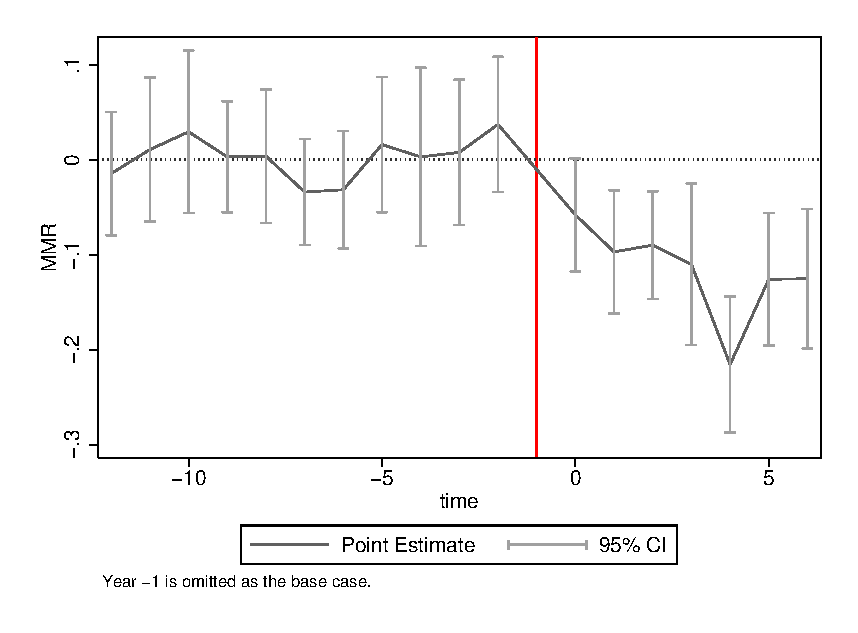
\includegraphics[scale=0.8]{./figures/eventMMR.eps}
\end{figure}
\end{frame}

\begin{frame}[IPREvent,plain]
\begin{figure}
\caption{Pneumonia (Placebo) Event Study Plot}
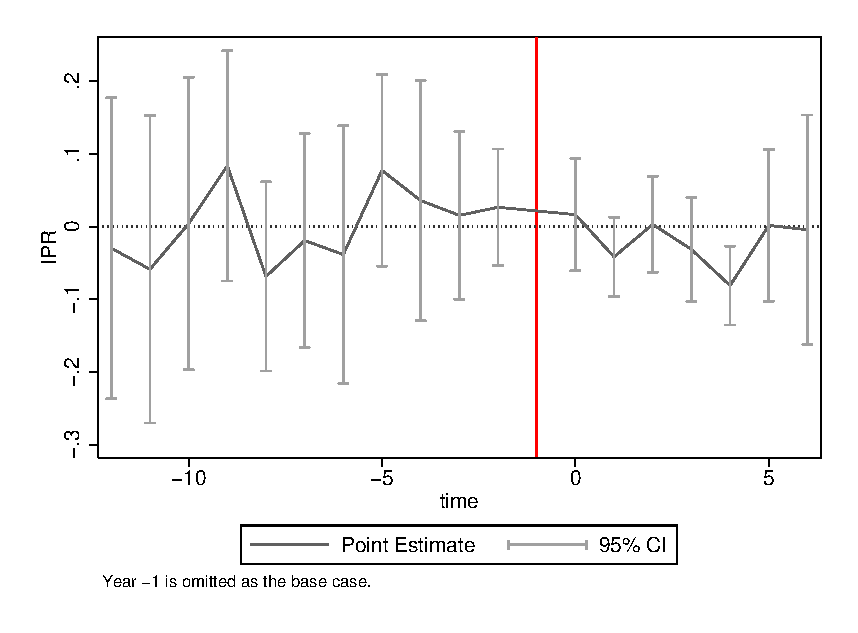
\includegraphics[scale=0.8]{./figures/eventIPR.eps}
\end{figure}
\end{frame}




\section{Quotas and Women in Parliament}
%********************************************************************************


\frame[plain]{
\begin{center}
\textbf{(2) Quotas and Women in Parliament}\\
\end{center}
}




\begin{frame}
\frametitle{(2) Quotas and Women in Parliament}
\begin{itemize}
\setlength{\itemsep}{15pt}
\item We have data from \url{www.quotaproject.org} on: (a) quota year, (b) quota type, (c) whether quota is in upper or lower chamber (if bicameral), and (d) what proportion of representation the quota is defined as.
\item The quota type is split between two types: guaranteed reserved seats (``reserved'') or a minimum proportion of female candidates  or candidates of both sex on the ballot (``candidates'')
\item The results here do \emph{not} include quotas at a sub-national level.
\end{itemize}
\end{frame}

\begin{frame}[label=Quotas]
\frametitle{Quotas: Estimation and results}
\begin{itemize}
\setlength{\itemsep}{15pt}
\item We first estimate a DID specification, in which we examine the effect of quota implementation on MMR in the following period.
\item Our baseline spec with year and country FEs is (\hyperlink{QuotaEstimates}{\textcolor{blue}{estimates}}):
\vspace{3mm}
\scriptsize
\begin{eqnarray}
log(MMR)_{ct} &= \alpha_0 + \alpha_1 Quota_{c,t-1} + \alpha_2 ln(GDP)_{c,t-1}  + \mu_c + \lambda_t + \varepsilon_{ct}  
\end{eqnarray}
\normalsize
%\item In our baseline specification we include year and country FEs, and controls the log of GDP per capita:
\item We then estimate a full event-study specification surrounding the implementation of quotas
\item We interact quota implementation with a full set of leads and lags, giving the following specification:
\scriptsize
\begin{eqnarray}
log(MMR)_{ct} = \alpha_0 + \sum_{j=1}^J \tau_{-j}*Quota_{c,t-j} + \sum_{k=1}^K \tau_{-k}*Quota_{c,t+k}+ \mu_c + \lambda_t + \varepsilon_{ct} \nonumber
\end{eqnarray}
\normalsize
\item In the spirit of Granger (1969) casuality, we should observe that if any effects from (1) are truly due to quotas, these should emerge only after the reform, and not in the pre-reform coefficients $\tau_{-j}.
\end{itemize}
\end{frame}



\begin{frame}[label=Quotas]
  \begin{figure}[htpb!]
    \begin{center}
      \centering
      \caption{Event Study: Women in Parliament and Reserved Seats}
      \includegraphics[scale=0.80]{./quotas/eventWomParl.eps}
      \label{fig:RWP}
    \end{center}
    \floatfoot{\textsc{Notes}: }
  \end{figure}
\end{frame}

\begin{frame}
  \begin{figure}[htpb!]
    \begin{center}
      \centering
      \caption{Event Study: log(Maternal Mortality Rate) and Reserved Seats}
      \includegraphics[scale=0.80]{./quotas/eventlnMDeath.eps}
      \label{fig:RMMR}
    \end{center}
    \floatfoot{\textsc{Notes}: }
  \end{figure}
    \begin{figure}[htpb!]
    \begin{center}
      \centering
      \caption{Event Study: Fertility Rate and Reserved Seats}
      \includegraphics[scale=0.80]{./quotas/eventFert.eps}
      \label{fig:RFert}
    \end{center}
    \floatfoot{\textsc{Notes}: }
  \end{figure}
\end{frame}

\begin{frame}
  \begin{figure}[htpb!]
    \begin{center}
      \centering
      \caption{Event Study: Women in Parliament and Candidate Lists}
      \includegraphics[scale=0.80]{./quotas/eventWomParl_cands.eps}
      \label{fig:RWP}
    \end{center}
    \floatfoot{\textsc{Notes}: }
  \end{figure}
\end{frame}

\begin{frame}
  \begin{figure}[htpb!]
    \begin{center}
      \centering
      \caption{Event Study: log(Maternal Mortality Rate) and Candidate Lists}
      \includegraphics[scale=0.80]{./quotas/eventlnMDeath_cands.eps}
      \label{fig:RMMR}
    \end{center}
    \floatfoot{\textsc{Notes}: }
  \end{figure}
\end{frame}


\begin{frame}[plain, label=QuotaEstimates]
\frametitle{Quotas: Estimation and results}
\begin{table}[htbp]\centering
\tiny
\def\sym#1{\ifmmode^{#1}\else\(^{#1}\)\fi}
\caption{Gender Quotas, Women in Parliament and Health}
\begin{tabular}{l*{6}{c}}
\toprule
                    &\multicolumn{3}{c}{Reserved Seats}             &\multicolumn{3}{c}{Candidate Quota}            \\\cmidrule(lr){2-4}\cmidrule(lr){5-7}
                    &\multicolumn{1}{c}{(1)}&\multicolumn{1}{c}{(2)}&\multicolumn{1}{c}{(3)}&\multicolumn{1}{c}{(4)}&\multicolumn{1}{c}{(5)}&\multicolumn{1}{c}{(6)}\\
                    &\multicolumn{1}{c}{\% Women}&\multicolumn{1}{c}{ln(MMR)}&\multicolumn{1}{c}{ln(TB)}&\multicolumn{1}{c}{\% Women}&\multicolumn{1}{c}{ln(MMR)}&\multicolumn{1}{c}{ln(TB)}\\
\midrule
Quota (reserved)    &       5.461***&      -0.080*  &       0.144   &               &               &               \\
                    &     [1.956]   &     [0.047]   &     [0.119]   &               &               &               \\
Quota (candidates)  &               &               &               &       3.946***&       0.050   &      -0.030   \\
                    &               &               &               &     [1.111]   &     [0.043]   &     [0.084]   \\
Constant            &       5.906   &       7.088***&       3.715***&       7.270   &       7.102***&       3.710***\\
                    &    [10.889]   &     [0.457]   &     [1.273]   &    [10.233]   &     [0.462]   &     [1.265]   \\
\midrule
R-Squared           &       0.456   &       0.586   &       0.401   &       0.452   &       0.585   &       0.398   \\
Observations        &        3846   &        3846   &        3819   &        3846   &        3846   &        3819   \\
Country and Year FE &Y&Y&Y&Y&Y&Y \\                       
\bottomrule\multicolumn{7}{p{10cm}}{\begin{tiny} The proportion of     
countries with reserved seats or a candidate list quota is  (respectively) 0.043 and 0.090. Standard errors   
clustered at the level of the country are reported in parentheses.    
***p-value$<$0.01, **p-value$<$0.05, *p-value$<$0.01 (\hyperlink{Quotas}{\textcolor{blue}{back})}.
\end{tiny}}\end{tabular}\end{table}
\end{frame}

%********************************************************************************

\section{Cross Country Evidence}

\frame[plain]{
\begin{center}
\textbf{(3) Cross-Country Evidence}\\
\end{center}
}




\begin{frame}[label=CC1]
\frametitle{(2) Cross-Country Evidence}
\begin{figure}[htpb!]
\centering
\begin{subfigure}{.5\textwidth}
  \centering
  \includegraphics[scale=0.3]{./newfigures/FLE_2010.png}
  \caption{Female LE and LGDP}
  \label{TWINfig:fertrend}
\end{subfigure}%
\begin{subfigure}{.5\textwidth}
  \centering
  \includegraphics[scale=0.3]{./newfigures/LEr_2010.png}
  \caption{Female LE advantage and LGDP}
  \label{TWINfig:eductrend}
\end{subfigure}
\end{figure}
\begin{itemize}
\item Simple trends suggest strong between LE and GDP
\item However, this is not the case for life expectancy \emph{ratio}
\end{itemize}
\end{frame}


\begin{frame}[label=CC2]
\frametitle{(2) Cross-Country Evidence}
\begin{figure}[htpb!]
\centering
\begin{subfigure}{.5\textwidth}
  \centering
  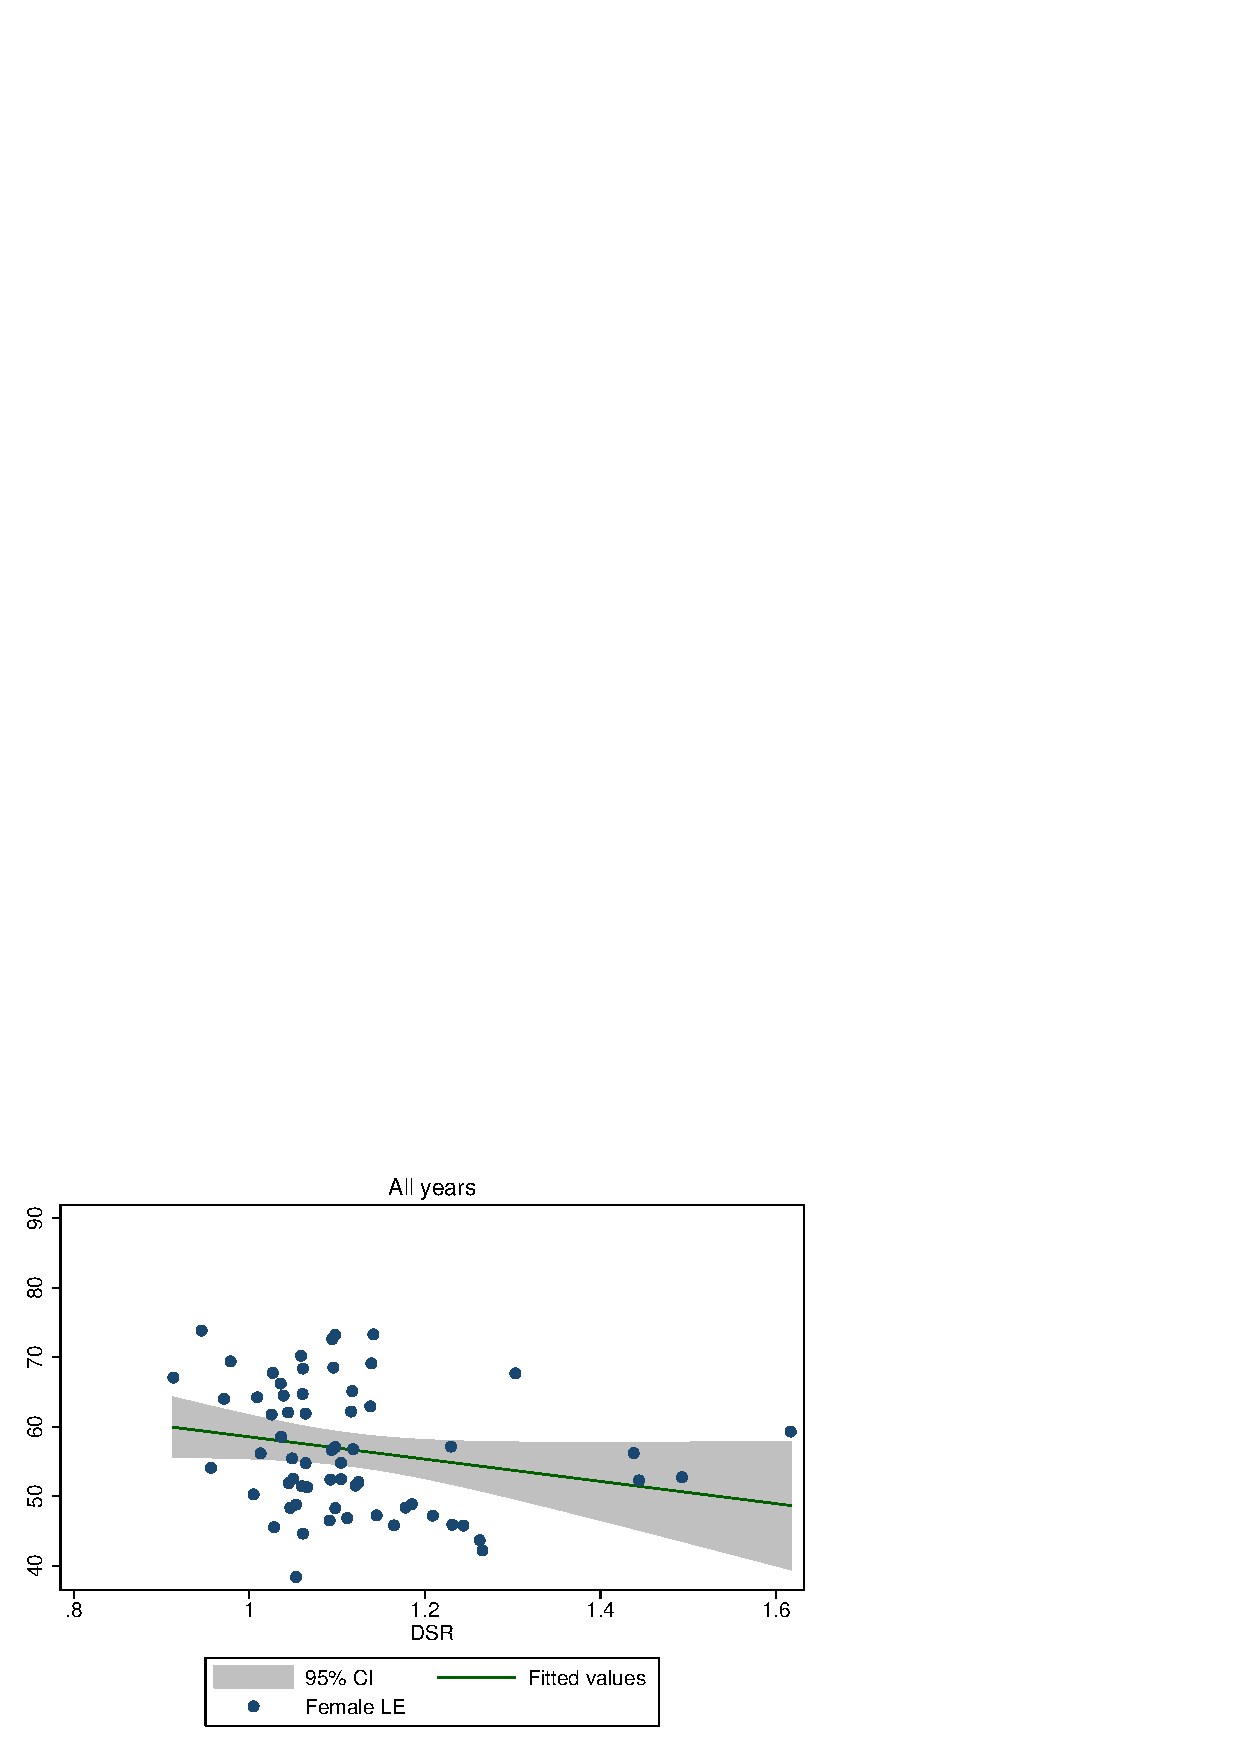
\includegraphics[scale=0.3]{./newfigures/lLEdesiredall.png}
  \caption{Female LE and DSR}
  \label{TWINfig:fertrend}
\end{subfigure}%
\begin{subfigure}{.5\textwidth}
  \centering
  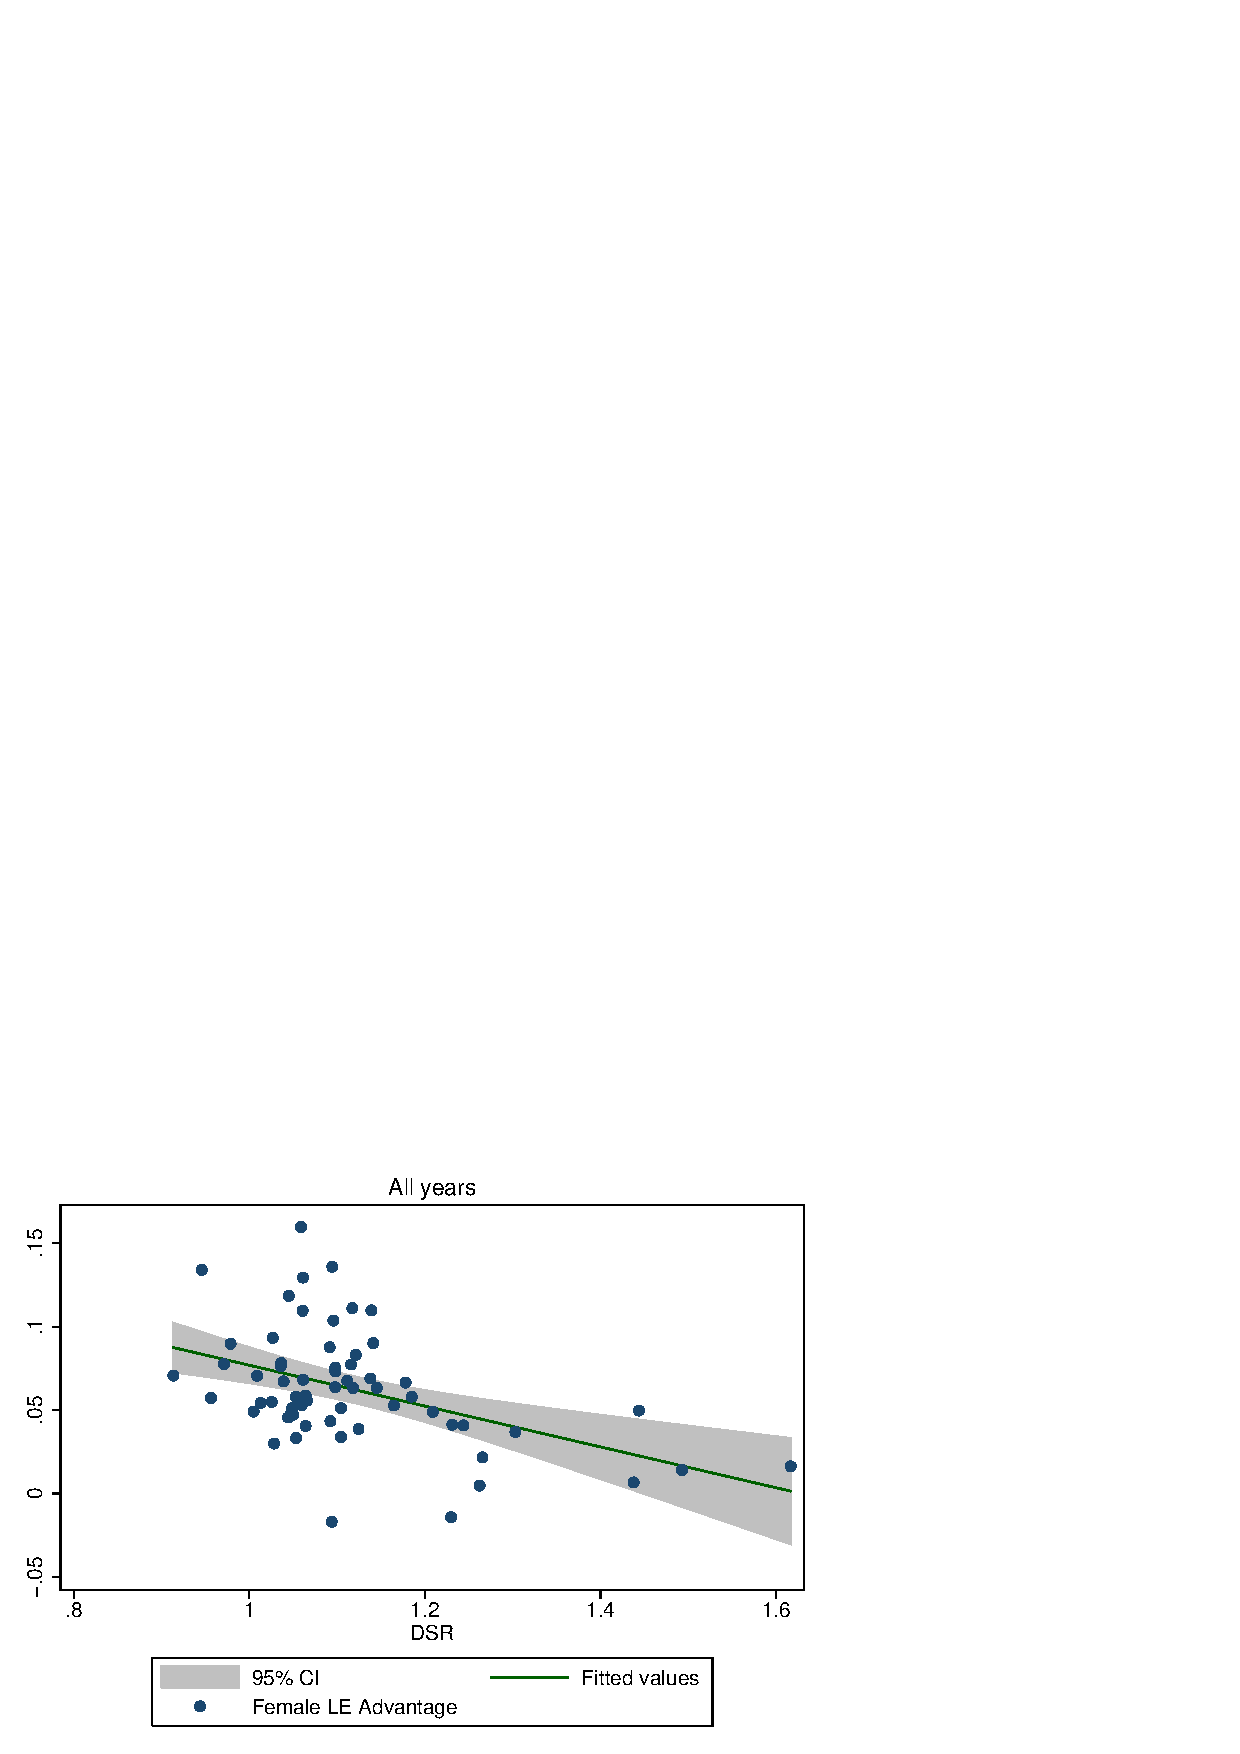
\includegraphics[scale=0.3]{./newfigures/lLErdesiredall.png}
  \caption{Female LE advantage and DSR}
  \label{TWINfig:eductrend}
\end{subfigure}
\end{figure}
\begin{itemize}
\item LE ratio much more strongly related to gender bias
\end{itemize}

\end{frame}


\begin{frame}[plain,label=MMRmap]
\begin{figure}[h!]
\centering
\includegraphics[scale= 0.4]{./figures/MMR}
\caption{MMR across the world (average across years 1990-2010).}
\end{figure}
%{\footnotesize \hyperlink{desc}{\textcolor{blue}{back}}}
\end{frame}


\begin{frame}
\frametitle{Cross country data sources}

\begin{table}[htbp]\centering
\def\sym#1{\ifmmode^{#1}\else\(^{#1}\)\fi}
\caption{Annual data  (with gaps)}
\scriptsize

						\begin{tabular}{lccc}
\hline
\hline
  Variable &     Source & n(Countries) &      Years \\
\hline
MMR (Deaths per 100,000 live births) &        WDI &        183 & 1990- 2015 \\

Subnational MMR calculated from microdata &        DHS &         45 &  1970-2010 \\

Life Expectancy (Male) &        WDI &        200 &  1960-2014 \\

Life Expectancy (Female) &        WDI &        200 &  1960-2015 \\

Life Expectancy Ratio (F/M) &        WDI &        200 &  1960-2016 \\

       GDP &        WDI &        190 &  1960-2015 \\

Tuberculosis Mortality Rate &        WDI &        191 &  1990-2015 \\

Desired Sex Ratio (M/F) &        DHS &         63 &  1960-2012 \\

Women's Political Rights &  Cingareli &        190 &  1981-2011 \\

Women's Economic Rights &  Cingareli &        190 &  1981-2011 \\

Women's Social Rights &  Cingareli &        190 &  1981-2004 \\
\hline
\end{tabular}  
\end{table}
\end{frame}


\begin{frame}
\begin{table}[htbp]\centering 
\scriptsize
\caption{Summary statistics \label{sumstat}}
\begin{tabular}{l c c c c c}\hline\hline
\multicolumn{1}{c}{\textbf{Variable}} & \textbf{Mean}
 & \textbf{Std. Dev.}& \textbf{Min.} &  \textbf{Max.} & \textbf{N}\\ 
\hline
Life Expectancy (Female)& 65.709 & 12.176 & 22.394 & 86.900 & 10629\\
Life Expectancy (Male) & 61.106 & 10.925 & 16.286 & 81.600 & 10629\\
LE ratio (F/M) & 1.074 & 0.036 & 0.963 & 1.375 & 10629\\
MMR & 251.57 & 357.733 & 3 & 2900 & 4758\\
Log GDP & 8.201 & 1.509 & 4.749 & 11.886 & 8342\\
Desired Sex Ratio (M/F) & 1.116 & 0.142 & 0.433 & 3 & 2997\\
Tuberculosis Mortality Rate & 21.559 & 32.145 & 0 & 283 & 4712\\
Women's Political Rights & 1.786 & 0.647 & 0 & 3 & 4830\\
Women's Economic Rights  & 1.323 & 0.697 & 0 & 3 & 4779\\
Women's Social Rights  & 1.235 & 0.84 & 0 & 3 & 3395\\
Women's Composite Rights 1& 0 & 1.436 & -3.435 & 3.882 & 3352\\
Women's Composite Rights 2 & 0 & 1.16 & -3.286 & 3.022 & 4766\\
%ngii grammar index& 0.46 & 0.498 & 0 & 1 & 6944\\
%sbii grammar index& 0.694 & 0.461 & 0 & 1 & 6944\\
%gaii grammar index& 0.692 & 0.462 & 0 & 1 & 5096\\
%gpii grammar index& 0.341 & 0.474 & 0 & 1 & 6888\\
%gt\_pronoun grammar index& 2.524 & 1.5 & 0 & 4 & 4592\\
%gii0 grammar index& 2.453 & 1.661 & 0 & 4 & 4816\\
%gii1 grammar index& 1.978 & 1.222 & 0 & 3 & 5096\\
%gii2 grammar index& 1.517 & 1.235 & 0 & 3 & 6496\\
\hline
\end{tabular}
\end{table}

\end{frame}


\begin{frame}[label=CC]
\frametitle{Conditional Analysis}
We estimate the following regression using panel data:
	\begin{equation}
		MMR_{it} = \alpha + \beta GenderBias_{it} + \gamma_i + \delta_t + 
               (\phi_i\times t) + \theta X_{it} + \varepsilon_{it}. \nonumber
	\end{equation}
\begin{itemize}
\setlength{\itemsep}{10pt}
	\item MMR is later replaced with the log ratio of female-male life expectancy.
  \item $GenderBias_{it}$ is measured as desired sex ratio of births, women's 
        rights and women's share of parliamentary seats.
	\item $\gamma$, $\delta$, $(\phi_i\times t)$ - country and year specific FE,
        country specific trends.  
  \item $X_{it}$ includes ln(GDP), interactions
	\item Standard errors are always clustered at the country level.
  \item We construct/collect data from various
        sources: WB, WHO, DHS
\end{itemize}
\end{frame}

\subsection{Desired Sex Ratio}

\begin{frame}
\frametitle{Gender Bias Proxied by Desired Sex Ratio}
\begin{itemize}
\setlength{\itemsep}{15pt}
\item We construct time profiles of the desired sex ratio of births at the individual level using the DHS
\item The DSR in, say, 1990, is the DSR reported by all women who were 15-25 years of age in 1990, irrespective of when their responses are elicited.
{\footnotesize \hyperlink{DSRMap}{\textcolor{blue}{See map}}}
\begin{itemize}
\item Low Son Preference countries: Dominican Republic (0.92); Haiti, Ukraine (0.94); Nicaragua (0.96), Colombia (0.99) 
\item Medium: Zimbabwe (1.08), Ghana (1.108), Tanzania (1.07) 
\item High: India (1.33), Nepal (1.42), Pakistan (1.59)
\end{itemize}
\item \hyperlink{DSRIMR}{\textcolor{blue}{We checked}} that DSR is strongly linked to excess girl infant mortality
\item Similar results hold when we use the life expectancy differential instead of MMR
\end{itemize}
\end{frame}


\begin{frame}[label=DSRanalysis]
\frametitle{Gender Bias Proxied by  Desired Sex Ratio} 
%\begin{table}[htbp]\centering
\def\sym#1{\ifmmode^{#1}\else\(^{#1}\)\fi}
\caption{MMR and Desired Sex Ratio (boys/girls)}
\scalebox{0.7}{
\begin{tabular}{l*{5}{c}}
\toprule
                    &\multicolumn{1}{c}{(1)}   &\multicolumn{1}{c}{(2)}   &\multicolumn{1}{c}{(3)}   &\multicolumn{1}{c}{(4)}   &\multicolumn{1}{c}{(5)}   \\
                    &     MMR \ \   &     MMR \ \   &     MMR \ \   &     MMR \ \   &     MMR \ \   \\
\midrule
Desired Sex Ratio   &       824.7** &       655.0** &       667.0** &       923.9***&      2627.7***\\
                    &     [329.4]   &     [299.3]   &     [286.5]   &     [252.9]   &     [617.9]   \\
ln(GDP)             &               &               &        40.9   &        12.4   &       318.5***\\
                    &               &               &      [48.5]   &      [49.8]   &     [119.6]   \\
Desired Sex Ratio$\times$ ln(GDP)&               &               &               &               &      -285.3***\\
                    &               &               &               &               &     [100.7]   \\
Constant            &      -476.0   &      -405.1   &      -712.6   &     -1514.3***&     -3371.0***\\
                    &     [358.9]   &     [325.8]   &     [494.2]   &     [483.9]   &     [734.5]   \\
\midrule
R-squared           &        0.09   &        0.92   &        0.92   &        0.93   &        0.93   \\
Observations        &         310   &         310   &         307   &         307   &         307   \\
 Country FE &&Y&Y&Y&Y\\ Year FE&&Y&Y&Y&Y\\ 
Desired Fertility&&&&Y&Y\\
\bottomrule\end{tabular}}\end{table}

\begin{table}[htbp]\centering
\def\sym#1{\ifmmode^{#1}\else\(^{#1}\)\fi}
\caption{MMR \& Desired Sex Ratio (boys/girls)  \label{MMRdsrNew}}
\scriptsize
\begin{tabular}{l*{5}{c}}
\hline\hline
            &\multicolumn{1}{c}{(1)}&\multicolumn{1}{c}{(2)}&\multicolumn{1}{c}{(3)}&\multicolumn{1}{c}{(4)}&\multicolumn{1}{c}{(5)}\\
            %&\multicolumn{1}{c}{indep1}&\multicolumn{1}{c}{indep2}&\multicolumn{1}{c}{indep3}&\multicolumn{1}{c}{indep3b}&\multicolumn{1}{c}{indep4}&\multicolumn{1}{c}{indep5}\\
\hline
Desired Sex Ratio  &       893.1         &       148.4         &       39.28         &       395.9\sym{***}&            4083.3\sym{***}\\
            &     (618.8)         &     (224.3)         &     (201.3)         &     (132.6)         &        (1477.7)         \\

log GDP        &                     &                     &      -88.90         &      -96.43\sym{*}  &              534.8\sym{**} \\
            &                     &                     &     (60.46)         &     (55.11)         &          (266.3)         \\

%Desired Fertility &                     &                     &                     &       308.2\sym{***}&                312.2\sym{***}\\
%            &                     &                     &                     &     (83.16)         &               (80.51)         \\

Desired Sex Ratio* log GDP    &                     &                     &                     &                     &          -585.9\sym{**} \\
            &                     &                     &                     &                     &         (246.8)         \\

%\_cons      &      -499.8         &       447.2\sym{*}  &      1176.7\sym{**} &      -428.2         &        -4422.6\sym{***}\\
%            &     (693.2)         &     (252.0)         &     (519.4)         &     (506.4)         &      (1617.2)         \\
\hline
\(N\)       &        1407         &        1407         &        1375         &        1375         &              1375         \\
r2          &                     &       0.407         &       0.409         &       0.520         &           0.542         \\
\hline
Country FE        &                     &    Y                 &      Y               &     Y         &               Y         \\
Year FE            &                     &    Y                 &      Y               &     Y         &             Y         \\
Desired Fertility &                     &                     &                     &       Y&             Y\\

\hline\hline
%\multicolumn{7}{l}{\footnotesize Standard errors in parentheses}\\
%\multicolumn{7}{l}{\footnotesize \sym{*} \(p<0.10\), \sym{**} \(p<0.05\), \sym{***} \(p<0.01\)}\\
\end{tabular}
\end{table}
\end{frame}

\subsection{Women's Rights}


\begin{frame}[label=WomensRights]
\frametitle{Gender Inequality II: Women's Rights}
\begin{itemize}
	\item Cingranelli et. al. 2013 data set on women's rights:
	 \vspace{4mm}
	\begin{itemize}
		%\item Political, Economic \& Social rights.
		\item Political - e.g. rights to vote, run for political office.
		 \vspace{4mm}
		\item Economic - e.g. equal pay for equal work, free choice of profession without the need to obtain a husband or male relative's consent.
		 \vspace{4mm}
		\item Social - e.g. equal inheritance, enter into marriage on a basis of equality with men.
				 \vspace{4mm}
		\item Women's Composite Rights 1 - First principal component of political, economic and social rights.
				 \vspace{4mm}
		\item Women's Composite Rights 2 - First principal component of political and economic social rights.

	\end{itemize}
\end{itemize}

\end{frame}

%\item Economic rights. %equal pay for equal work; free choice of profession or employment without the need to obtain a husband or male relative's consent; gainful employment without the need to obtain a husband or male relative's consent; equality in hiring and promotion practices; job security (maternity leave, unemployment benefits, no arbitrary firing or layoffs, etc...); non-discrimination by employers; be free from sexual harassment in the workplace; work at night; work in occupations classified as dangerous; work in the military and the police force.  
		%\item Social rights.  %equal inheritance; enter into marriage on a basis of equality with men; travel abroad; obtain a passport; confer citizenship to children or a husband; initiate a divorce;  own, acquire, manage, and retain property brought into marriage; participate in social, cultural, and community activities; an education; choose a residence/domicile; freedom from female genital mutilation of children and of adults without their consent; and the freedom from forced sterilization.




\begin{frame}
\frametitle{Gender Bias Measured by  Women's Rights  (Cingranelli et al., 2013)}
%\input{./tables/rightsMMR.tex}
\begin{table}[htbp]\centering
\def\sym#1{\ifmmode^{#1}\else\(^{#1}\)\fi}
\caption{Maternal Mortality and Women's Rights \label{MMRbWRightWDINew}}
\scriptsize
\begin{tabular}{l*{6}{c}}
\hline\hline
            &\multicolumn{1}{c}{(1)}&\multicolumn{1}{c}{(2)}&\multicolumn{1}{c}{(3)}&\multicolumn{1}{c}{(4)}&\multicolumn{1}{c}{(5)}&\multicolumn{1}{c}{(6)}\\
            %&\multicolumn{1}{c}{indep0}&\multicolumn{1}{c}{indep1}&\multicolumn{1}{c}{indep2}&\multicolumn{1}{c}{indep3}&\multicolumn{1}{c}{indep4}&\multicolumn{1}{c}{indep5}\\
\hline
Political Rights      &      -22.73\sym{*}  &      -20.91         &      -23.12         &      -346.6\sym{***}&      -350.9\sym{***}&      -313.9\sym{***}\\
            &     (13.02)         &     (13.00)         &     (14.64)         &     (78.43)         &     (84.99)         &     (76.09)         \\

log GDP         &      -99.44\sym{***}&      -39.64         &      -31.33         &      -105.5\sym{***}&      -97.63\sym{***}&      -134.8\sym{***}\\
            &     (17.39)         &     (32.77)         &     (33.76)         &     (33.23)         &     (34.89)         &     (40.12)         \\

%Democracy       &                     &                     &      -7.870\sym{*}  &                     &      -5.915\sym{*}  &      -73.19\sym{***}\\
%            &                     &                     &     (4.223)         &                     &     (3.572)         &     (22.82)         \\

Rights*log GDP  &                     &                     &                     &       40.46\sym{***}&       40.73\sym{***}&       36.57\sym{***}\\
            &                     &                     &                     &     (8.693)         &     (9.335)         &     (8.357)         \\

%Democracy * lGDP   &                     &                     &                     &                     &                     &       9.241\sym{***}\\
%            &                     &                     &                     &                     &                     &     (2.795)         \\

%\_cons      &      1164.1\sym{***}&       679.7\sym{**} &       654.1\sym{**} &      1206.2\sym{***}&      1173.5\sym{***}&      1398.5\sym{***}\\
%            &     (160.6)         &     (269.3)         &     (277.2)         &     (278.0)         &     (295.3)         &     (328.0)         \\
\hline
\(N\)       &        3424         &        3424         &        3135         &        3424         &        3135         &        3135         \\
r2          &                     &       0.254         &       0.273         &       0.348         &       0.362         &       0.397         \\
\hline\hline
Economic Rights      &       10.38         &       11.71         &       10.90         &      -36.20         &      -37.35         &      -28.21         \\
            &     (6.932)         &     (7.288)         &     (7.589)         &     (49.19)         &     (51.17)         &     (48.99)         \\

log GDP         &      -99.51\sym{***}&      -38.69         &      -28.26         &      -43.26         &      -32.98         &      -87.23\sym{**} \\
            &     (17.85)         &     (33.61)         &     (34.48)         &     (35.11)         &     (35.93)         &     (39.67)         \\

%Democracy       &                     &                     &      -7.533\sym{*}  &                     &      -7.517\sym{*}  &      -90.67\sym{***}\\
%            &                     &                     &     (4.186)         &                     &     (4.200)         &     (28.18)         \\

Rights*log GDP  &                     &                     &                     &       5.740         &       5.774         &       4.432         \\
            &                     &                     &                     &     (5.224)         &     (5.417)         &     (5.183)         \\

%Democracy * lGDP   &                     &                     &                     &                     &                     &       11.47\sym{***}\\
%            &                     &                     &                     &                     &                     &     (3.481)         \\

%\_cons      &      1115.4\sym{***}&       622.4\sym{**} &       575.4\sym{**} &       659.0\sym{**} &       613.1\sym{**} &       965.0\sym{***}\\
%            &     (157.5)         &     (276.9)         &     (281.3)         &     (289.3)         &     (293.1)         &     (317.1)         \\
\hline
\(N\)       &        3412         &        3412         &        3124         &        3412         &        3124         &        3124         \\
r2          &                     &       0.250         &       0.266         &       0.252         &       0.268         &       0.324         \\
\hline
\hline
Country FE        &                     &    Y                 &      Y               &     Y         &           Y          &     Y         \\
Year FE            &                     &    Y                 &      Y               &     Y         &           Y          &     Y         \\
Democracy       &                     &                     &     Y &                     &      Y  &      Y\\
Democracy*log GDP   &                     &                     &                     &                     &                     &      Y\\

\hline
%\multicolumn{7}{l}{\footnotesize Standard errors in parentheses}\\
%\multicolumn{7}{l}{\footnotesize \sym{*} \(p<0.10\), \sym{**} \(p<0.05\), \sym{***} \(p<0.01\)}\\
\end{tabular}
\end{table}
\end{frame}



\begin{frame}
\frametitle{Gender Bias Measured by Women's Composite Rights}
\begin{table}[htbp]\centering
\def\sym#1{\ifmmode^{#1}\else\(^{#1}\)\fi}
\scriptsize
\caption{Maternal Mortality and Women's Composite Rights \label{MMRWRight3}}
\begin{tabular}{l*{6}{c}}
\hline\hline
            &\multicolumn{1}{c}{(1)}&\multicolumn{1}{c}{(2)}&\multicolumn{1}{c}{(3)}&\multicolumn{1}{c}{(4)}&\multicolumn{1}{c}{(5)}&\multicolumn{1}{c}{(6)}\\
            %&\multicolumn{1}{c}{indep0}&\multicolumn{1}{c}{indep1}&\multicolumn{1}{c}{indep2}&\multicolumn{1}{c}{indep3}&\multicolumn{1}{c}{indep4}&\multicolumn{1}{c}{indep5}\\
\hline
\multicolumn{1}{p{2cm}}{Political,Economic, }       &      -4.276         &      -3.094         &      -4.187         &      -122.3\sym{***}&      -126.0\sym{***}&      -115.4\sym{***}\\
  Social Rights          &     (4.518)         &     (4.662)         &     (4.827)         &     (32.68)         &     (33.64)         &     (31.59)         \\

log GDP        &      -101.7\sym{***}&      -37.54         &      -42.46         &      -32.60         &      -36.96         &      -70.65\sym{*}  \\
            &     (20.04)         &     (36.27)         &     (36.59)         &     (35.10)         &     (35.10)         &     (39.69)         \\

%democ       &                     &                     &      -2.130         &                     &      -1.713         &      -51.66\sym{**} \\
%            &                     &                     &     (2.340)         &                     &     (2.306)         &     (19.83)         \\

Rights*log GDP    &                     &                     &                     &       14.84\sym{***}&       15.14\sym{***}&       13.80\sym{***}\\
            &                     &                     &                     &     (3.694)         &     (3.796)         &     (3.540)         \\

%Democracy * log GDP   &                     &                     &                     &                     &                     &       7.009\sym{***}\\
%            &                     &                     &                     &                     &                     &     (2.589)         \\

%\_cons      &      1143.2\sym{***}&       628.8\sym{**} &       675.4\sym{**} &       576.7\sym{**} &       615.7\sym{**} &       831.0\sym{***}\\
%            &     (172.3)         &     (293.8)         &     (297.1)         &     (283.7)         &     (284.6)         &     (310.6)         \\
\hline
\(N\)       &        2111         &        2111         &        1972         &        2111         &        1972         &        1972         \\
r2          &                     &       0.215         &       0.215         &       0.265         &       0.269         &       0.299         \\
\hline\hline

\multicolumn{1}{p{2cm}}{Political \& }       &      -3.590         &      -2.147         &      -3.371         &      -184.8\sym{***}&      -183.0\sym{***}&      -160.6\sym{***}\\
 Economic Rights          &     (5.952)         &     (6.161)         &     (6.956)         &     (43.70)         &     (47.74)         &     (43.13)         \\

log GDP        &      -96.69\sym{***}&      -37.17         &      -27.16         &      -22.23         &      -12.95         &      -63.28\sym{*}  \\
            &     (17.87)         &     (33.78)         &     (34.56)         &     (31.40)         &     (32.30)         &     (35.64)         \\

%democ       &                     &                     &      -7.795\sym{*}  &                     &      -6.608\sym{*}  &      -79.60\sym{***}\\
            &                     &                     &     (4.274)         &                     &     (3.914)         &     (25.41)         \\

Rights*log GDP    &                     &                     &                     &       22.28\sym{***}&       21.98\sym{***}&       19.29\sym{***}\\
            &                     &                     &                     &     (4.843)         &     (5.237)         &     (4.693)         \\

%Democracy * lgdp   &                     &                     &                     &                     &                     &       10.04\sym{***}\\
 %           &                     &                     &                     &                     &                     &     (3.113)         \\

%\_cons      &      1103.0\sym{***}&       621.9\sym{**} &       578.0\sym{**} &       489.0\sym{*}  &       444.8\sym{*}  &       776.0\sym{***}\\
%            &     (156.0)         &     (274.9)         &     (278.7)         &     (254.8)         &     (258.9)         &     (282.0)         \\
\hline
\(N\)       &        3400         &        3400         &        3113         &        3400         &        3113         &        3113         \\
r2          &                     &       0.245         &       0.263         &       0.313         &       0.327         &       0.369         \\
\hline
Country FE        &                     &    Y                 &      Y               &     Y         &           Y          &     Y         \\
Year FE            &                     &    Y                 &      Y               &     Y         &           Y          &     Y         \\
Democracy       &                     &                     &     Y &                     &      Y  &      Y\\
Democracy*log GDP   &                     &                     &                     &                     &                     &      Y\\

\hline
%\multicolumn{7}{l}{\footnotesize Standard errors in parentheses}\\
%\multicolumn{7}{l}{\footnotesize \sym{*} \(p<0.10\), \sym{**} \(p<0.05\), \sym{***} \(p<0.01\)}\\
\end{tabular}
\end{table}
\end{frame}

\begin{frame}
\frametitle{Gender bias has large effects on women's health :}
%\vspace{4mm}
\begin{itemize}
	\item A 1 s.d. increase in son preference results in:
	%\vspace{4mm}
	\begin{itemize}
		\item 48 additional maternal deaths per 100k live births which is 10\% of the MMR mean and 11\% of the s.d.
		%\vspace{4mm}
		\item A 62\% reduction in a girl child's survival advantage.  
		\item A 1 s.d.increase in women's political rights leads to 9 fewer maternal deaths per 100k live births which is 3.42\% of the mean and 2.48\% of the s.d. in an average GDP country
    %\vspace{4mm}
	\end{itemize}
	%\vspace{4mm}
	\item Comparing reductions in MMR in early- and late-suffrage states following the arrival of sulfanide drugs in the USA:
		
\begin{itemize}
		\item Early suffrage states in the USA reduced MMR by nearly 10 percentage points more than late suffrage states
    %\vspace{4mm}
		\item In comparative terms, this is approximately \emph{double} the effect seen in late-suffrage states
\end{itemize}
		%\vspace{4mm}

		\item A 1 s.d. increase in quotas leads to
		\begin{itemize}
		\item an increase of 8.4\% of the mean and 11.33\% of the SD of \% of women in parliament.
    %\vspace{4mm}
		\item a fall of 33.6\% of the mean and 8\% of the SD of log of MMR.
\end{itemize}
\end{itemize}
\end{frame}



\subsection{Grammatical Gender}
\frame{
\frametitle{Gender Bias and Grammatical Gender}
\begin{equation}
MMR_{it} = \beta_0 + \beta_1 GII_i + \beta_2 PercentLang_i + X_{it} + X_i  + \nu_{it} \nonumber
\end{equation}
\begin{itemize}
\setlength{\itemsep}{15pt}
  \item GII is highly pre-determined but it does not vary over time. So we
        include continent FE rather than country FE.
	\item The idea is that grammatical gender reflects gender attitudes in society
	\begin{itemize}
		\item Maternity leave policy differences (Givati \& Troiano, 2012).
		\item Female labour force and political participation (Gay et al. 2013).
	\end{itemize}
%\begin{enumerate}
%\item Sex-Based Intensity Index (sbii) 
%\item Number Gender Intensity Index (ngii)
%\item Gender Assignment Intensity Index (gaii) 
%\item Gender Pronouns Intensity Index (gpii) 
%\item gii0 = ngii + sbii + gaii + gpii
%\item gii1 = ngii + sbii + gaii
%\item gii2 = ngii + sbii + gpii
%\item gtroiano = number of cases of gender differentiated pronouns.
%\end{enumerate}
\item Example: gender differentiated personal pronouns: 
	\begin{itemize}
		\item English (``He", ``She")  
		\item Spanish (\textit{``El"}, \textit{``Ella"}; \textit{``Ellos"},
          \textit{``Ellas"};\textit{``Nosotros"}, \textit{``Nosotras"};
          \textit{``Vosotros"}, \textit{``Vosotras"})
	\end{itemize}
\end{itemize}
}


\subsection{Grammatical Gender}
\frame{
\frametitle{Gender Bias and Grammatical Gender}
\begin{itemize}
\setlength{\itemsep}{15pt}
  \item The different measures used are:
\begin{enumerate}
\item Sex-Based Intensity Index (sbii) 
\item Number Gender Intensity Index (ngii)
\item Gender Assignment Intensity Index (gaii) 
\item Gender Pronouns Intensity Index (gpii) 
\item gii0 = ngii + sbii + gaii + gpii
\item gii1 = ngii + sbii + gaii
\item gii2 = ngii + sbii + gpii
\item gtroiano = number of cases of gender differentiated pronouns.
\end{enumerate}
\begin{table}[htbp]\centering 
\scriptsize
\caption{Summary statistics \label{sumstat}}
\begin{tabular}{l c c c c c}\hline\hline
\multicolumn{1}{c}{\textbf{Variable}} & \textbf{Mean}
 & \textbf{Std. Dev.}& \textbf{Min.} &  \textbf{Max.} & \textbf{N}\\ 
\hline
Number Gender Intensity Index & 0.46 & 0.498 & 0 & 1 & 6944\\
Sex-Based Intensity Index& 0.694 & 0.461 & 0 & 1 & 6944\\
Gender Assignment Intensity Index& 0.692 & 0.462 & 0 & 1 & 5096\\
Gender Pronouns Intensity Index & 0.341 & 0.474 & 0 & 1 & 6888\\
gtroiano& 2.524 & 1.5 & 0 & 4 & 4592\\
gii0 & 2.453 & 1.661 & 0 & 4 & 4816\\
gii1 & 1.978 & 1.222 & 0 & 3 & 5096\\
gii2 & 1.517 & 1.235 & 0 & 3 & 6496\\
\hline
\end{tabular}
\end{table}
\end{itemize}
}

\begin{frame}
\frametitle{MMR and Gender Intensity of Language Measures}
%\input{./tables/MMRGII.tex}
\begin{table}[htbp]\centering
\def\sym#1{\ifmmode^{#1}\else\(^{#1}\)\fi}
\caption{MMR and Gender Intensity of Language Measures}
\scalebox{0.5}{
\begin{tabular}{l*{8}{c}}
\toprule
\textsc{Dep Var}:   &\multicolumn{1}{c}{(1)}&\multicolumn{1}{c}{(2)}&\multicolumn{1}{c}{(3)}&\multicolumn{1}{c}{(4)}&\multicolumn{1}{c}{(5)}&\multicolumn{1}{c}{(6)}&\multicolumn{1}{c}{(7)}&\multicolumn{1}{c}{(8)}\\
 MMR                &\multicolumn{1}{c}{NGII}&\multicolumn{1}{c}{SBII}&\multicolumn{1}{c}{GPII}&\multicolumn{1}{c}{GAII}&\multicolumn{1}{c}{GII0}&\multicolumn{1}{c}{GII1}&\multicolumn{1}{c}{GII2}&\multicolumn{1}{c}{GTroiano}\\
\midrule
\multicolumn{9}{l}{\textsc{Panel A: No Interaction}}\\
Gender Intensity Index&       49.46\sym{**} &       74.83\sym{**} &       88.22\sym{***}&       59.25         &       28.71\sym{**} &       36.36\sym{***}&       26.87\sym{**} &      -3.505         \\
            &     (21.84)         &     (33.97)         &     (29.38)         &     (38.07)         &     (11.96)         &     (13.33)         &     (13.10)         &     (8.525)         \\
ln(GDP)             &      -70.70\sym{***}&      -71.43\sym{***}&      -78.61\sym{***}&      -71.20\sym{***}&      -75.02\sym{***}&      -72.07\sym{***}&      -68.95\sym{***}&      -71.37\sym{***}\\
            &     (16.55)         &     (16.53)         &     (23.98)         &     (17.49)         &     (24.74)         &     (23.70)         &     (17.35)         &     (19.09)         \\
R-squared           &       0.740         &       0.744         &       0.758         &       0.746         &       0.745         &       0.757         &       0.733         &       0.620         \\
Observations        &        2914         &        2914         &        2103         &        2849         &        2012         &        2103         &        2745         &        1928         \\
\\ \multicolumn{9}{l}{\textsc{Panel B: GDP Interaction}}\\
Gender Intensity Index&       447.1\sym{***}&       297.1\sym{*}  &       740.5\sym{***}&       501.2\sym{**} &       227.7\sym{***}&       274.1\sym{***}&       193.4\sym{***}&       140.5\sym{**} \\
            &     (130.4)         &     (150.1)         &     (128.8)         &     (195.2)         &     (45.35)         &     (57.27)         &     (63.21)         &     (67.04)         \\
GII $\times$ ln(GDP)&      -45.10\sym{***}&      -26.15\sym{*}  &      -77.00\sym{***}&      -51.44\sym{**} &      -24.35\sym{***}&      -29.44\sym{***}&      -20.00\sym{***}&      -15.63\sym{**} \\
            &     (13.28)         &     (15.41)         &     (14.57)         &     (19.88)         &     (5.163)         &     (6.833)         &     (6.796)         &     (7.032)         \\
ln(GDP)             &      -45.81\sym{**} &      -50.68\sym{**} &      -31.48         &      -55.07\sym{***}&      -7.283         &      -10.97         &      -33.48         &      -33.09         \\
            &     (17.64)         &     (22.39)         &     (21.96)         &     (18.45)         &     (24.13)         &     (23.21)         &     (20.61)         &     (23.29)         \\
\midrule
R-squared           &       0.756         &       0.748         &       0.788         &       0.756         &       0.768         &       0.779         &       0.745         &       0.639         \\
Observations        &        2914         &        2914         &        2103         &        2849         &        2012         &        2103         &        2745         &        1928         \\
\bottomrule\end{tabular}}\end{table}
\end{frame}


\subsection{Plough Use}
\begin{frame}[label=PlowSlide]
\frametitle{Plough use and reduction in maternal mortality}
\begin{equation}
MMR_{it} = \beta_0 + \beta_1 plough_i + \beta_2 plough_i*lgdp_i + X_{it} + X_i  + \nu_{it} \nonumber
\end{equation}
\begin{itemize}
\setlength{\itemsep}{15pt}
  \item $plough_i$ comes from Alesina et al. (2013) indicating historical plough use in country $i$
	\item Also highly pre-determined but it does not vary over time. 	So we
        include continent FE rather than country FE.
	\item However, in some specs we include country and year FE with only interaction of plough with either Log GDP or Women in Parliament.		
	\item In the \hyperlink{PlowResults}{\textcolor{blue}{specs}}  using country and year FE, we find that both GDP and women in parliament have a smaller effect on MMR in societies which traditionally practiced plough agriculture. 	
\end{itemize}
\end{frame}



\begin{frame}[label=PlowResults]
\frametitle{Plough use and reduction in maternal mortality}
\begin{table}[htbp]\centering
\def\sym#1{\ifmmode^{#1}\else\(^{#1}\)\fi}
\scriptsize
\caption{MMR and plough use}
\begin{tabular}{l*{4}{c}}
\hline\hline
            &\multicolumn{1}{c}{(1)}&\multicolumn{1}{c}{(2)}&\multicolumn{1}{c}{(3)}&\multicolumn{1}{c}{(4)}\\
            %&\multicolumn{1}{c}{est1}&\multicolumn{1}{c}{est2}&\multicolumn{1}{c}{est3}&\multicolumn{1}{c}{est4}&\multicolumn{1}{c}{est5}\\
\hline
Plough use        &      -173.9\sym{***}&      -28.32         &      -410.7\sym{*}  &                           \\
            &     (62.75)         &     (44.07)         &     (221.1)         &                                    \\

Log GDP        &                     &      -99.47\sym{***}&      -133.2\sym{***}&      -195.6\sym{***}\\
            &                     &     (19.87)         &     (24.22)         &     (34.37)               \\

Plough * Log GDP   &                     &                     &       46.70\sym{**} &       206.3\sym{***}               \\
            &                     &                     &     (23.55)         &     (48.50)                         \\

            &                     &                     &                     &                         \\
\hline
\(N\)       &        4654         &        3865         &        3865         &        4415               \\
r2          &       0.514         &       0.711         &       0.715         &       0.336                \\
\hline\hline
%\multicolumn{5}{l}{\footnotesize * \(p<0.10\), ** \(p<0.05\), *** \(p<0.01\)}\\
\multicolumn{5}{p{8cm}}{\footnotesize The dependent variables is MMR (deaths per 100,000 births) from WDI. The first 3 columns use continent and decade fixed effects (but no country or year fixed effects) along with controls for log population; percentage of protestants, muslims and catholics; and proportion of country that's tropical. In the final column we use country and year fixed effects instead.}\\
\end{tabular}
\end{table}
 %\hyperlink{PlowSlide}{\textcolor{blue}{Back}}  
\end{frame}


%********************************************************************************
\section{Sub-national evidence from Africa}

\frame[plain]{
\begin{center}
\textbf{(3) Sub-national Variation in Gender Bias}\\
\end{center}
}

\begin{frame}
\frametitle{(3) Sub-national Variation in Gender Bias}
Cross-country evidence above provides suggestive evidence, but concerns given
that language is fixed by country, and potential for unobservables in panel 
results
\vspace{5mm}
\begin{itemize}
\setlength{\itemsep}{20pt}
  \item We use time and regional variation in MMR to examine whether historically
        more biased regions progress less towards improvements in female health
        outcomes
  \item Examine protestant missions (Nunn, 2012)
  \item We observe local (sub-national) variation in these variables, so can
        control for country-specific factors (FEs)
\end{itemize}
\end{frame}



\begin{frame}[label=missions]
\frametitle{(3) Sub-national Variation in Gender Bias}
Effect of Protestant missions: evidence suggesting that 
Protestant missions historically were open to women's education(Nunn, 2013) %, while Catholic missions promoted male education
\vspace{2mm}
\begin{itemize}
\setlength{\itemsep}{15pt}
\item We follow an identical specification (wrt controls) as Nunn
\item \hyperlink{MissionsTab}{\textcolor{blue}{We find}} that in both the 
      Nunn (Afrobarometer) sample and the full Africa DHS sample (\hyperlink{MissionsMap}{\textcolor{blue}{Missionary locations}}):
\begin{itemize}
\item Areas with more Protestant missions have lower MMR today
\item Areas with more Protestant missions have higher women's education today
%\item Areas with more Catholic missions have higher men's education today
\end{itemize}
\end{itemize}
\end{frame}

\begin{frame}[label=MissionsMap]
\vspace{1cm}
%\input{./figures/Missions_map.png}
\begin{figure}[h!]
\centering
\includegraphics[scale= .35]{./figures/Missions_map.png}
\caption{Missionaries in Africa }
%\caption{Missionaries in Africa {\footnotesize \hyperlink{missions}{\textcolor{blue}{(back)}}}}
\end{figure}
\vspace{1cm}

\end{frame}

\begin{frame}[label=MissionsTab]
\vspace{1cm}
\input{./tables/missions.tex}
\vspace{1cm}
%{\footnotesize \hyperlink{missions}{\textcolor{blue}{back}}}
\end{frame}

%********************************************************************************
\section{Placebo}

\frame[plain]{
\begin{center}
\textbf{(4) Gender Neutral Placebo Tests}\\
\end{center}
}


\begin{frame}[label=placebos]
\frametitle{(4) Gender Neutral Placebo Tests}
\begin{itemize}
\setlength{\itemsep}{15pt}
  \item Tuberculosis is a ``gender neutral'' infectious disease
  \item Frequently occurring (around 9 million cases in 2013). Incidence ranges
        from less than 10 cases per 100,000 people, to greater than 1,000 per
        100,000 (ie a range very similar to MMR)
  \item We estimate the same set of specifications with the same measures of
        gender bias, replacing MMR with TB.
  \item Same tests replacing MMR with TB largely lead to null results:
  \begin{itemize}
    \item \hyperlink{placebo1}{\textcolor{blue}{Women's Rights as gender
                                                inequality proxy}}
    \item \hyperlink{placebo2}{\textcolor{blue}{Desired Sex Ratio}}
    \item \hyperlink{placebo3}{\textcolor{blue}{Gender inequality embedded in
                                                language}}
  \end{itemize}
\end{itemize}
\end{frame}


%********************************************************************************
\section{Conclusion}
\begin{frame}
\frametitle{Discussion and Conclusions}
\begin{itemize}
\setlength{\itemsep}{12pt}
	\item Preventable maternal mortality is still very high in many developing 
        countries, even after falling by almost 50\% since 1990.
	\item It exhibits substantial cross-country variation conditional on income.
	\item We show that there is a consistent relationship whereby MMR conditional 
        on income varies systematically with measures of gender prejudice.
	\item Female life expectancy advantage behaves like MMR in this regard
	\item This result is, in general, robust to alternative measures of gender 
        prejudice
	\item It is evident within countries over time and in the cross-section of
        countries, it was evident in 1930s America and is evident in today's
        poorer countries.
\end{itemize}
\end{frame}



%********************************************************************************
%********************************************************************************
%*** APPENDICES
%********************************************************************************
%********************************************************************************

\section{Appendices}

\begin{frame}[plain]
\begin{center}
\textbf{Appendices}
\end{center}
\end{frame}


\begin{frame}[label=Yentl]
\frametitle{The Yentl Syndrome}
From the New England Journal of Medicine: \\
\vspace{4mm}
\textit{Yentl, the 19th-century heroine of Isaac Bashevis Singer's short story, 
had to disguise herself as a man to attend school and study the Talmud. Being 
``just like a man'' has historically been a price women have had to pay for 
equality. Being different from men has meant being second-class and less than 
equal for most of recorded time and throughout most of the world. It may therefore 
be sad, but not surprising, \hyperlink{intro}{\textcolor{red}{that women have all 
too often been treated less than equally in social relations, political endeavors, 
business, education, research, and health care.}}}\\
\end{frame}



\begin{frame}[plain,label=DDreg]
\input{./tables/mechanism.tex}
{\footnotesize \hyperlink{USA}{\textcolor{blue}{back}}}
\end{frame}


\begin{frame}[plain,label=ptrends]
\begin{figure}[h!]
\centering
\caption{Trends in ln(MMR)}
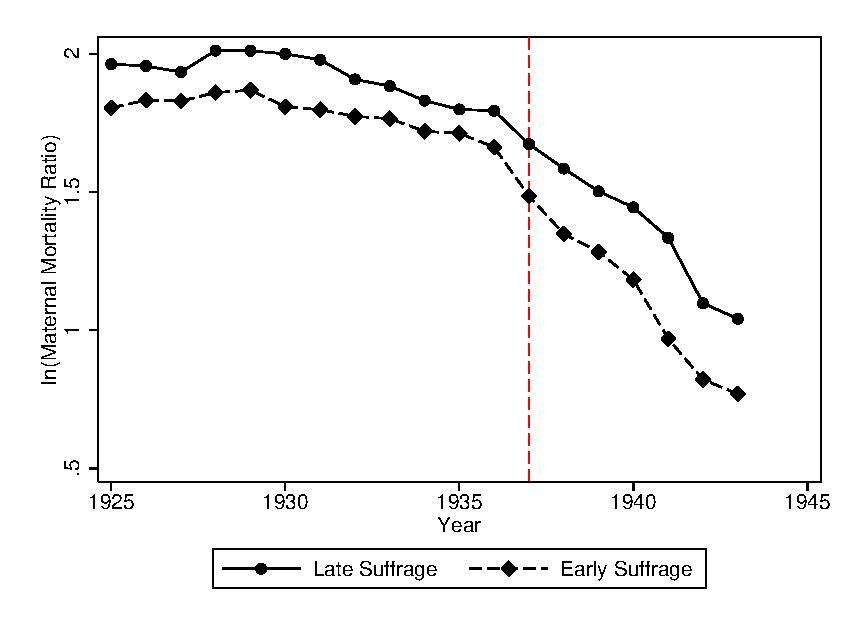
\includegraphics[scale=0.67]{./figures/MMRtrends.eps}
\end{figure}
{\footnotesize \hyperlink{USA}{\textcolor{blue}{back}}}
\end{frame}

\begin{frame}[plain,label=ptrends]
\begin{figure}[h!]
\centering
\caption{Trends in ln(IPR)}
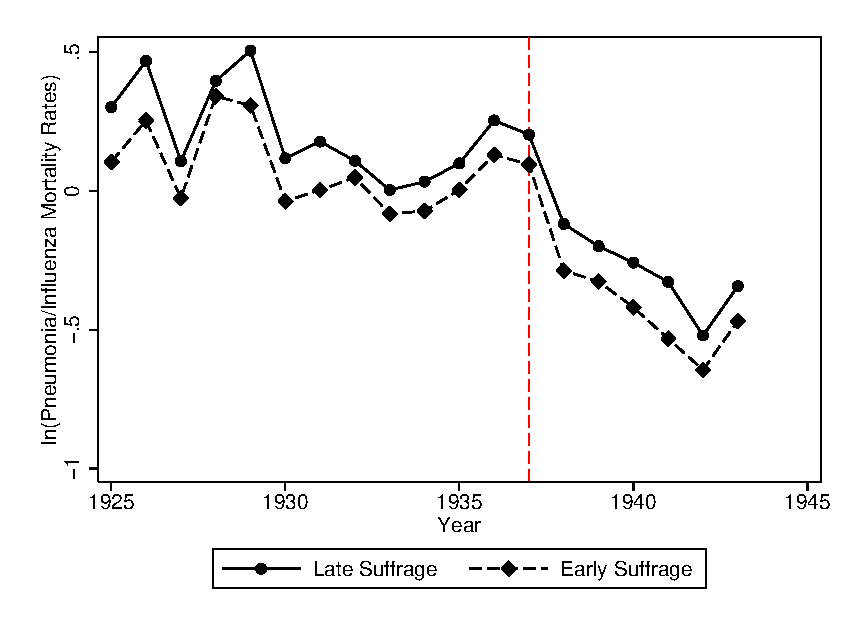
\includegraphics[scale=0.67]{./figures/IPRtrends.eps}
\end{figure}
{\footnotesize \hyperlink{USA}{\textcolor{blue}{back}}}
\end{frame}







\begin{frame}[label=placebo1]
%\input{./tables/rightstb.tex}
\begin{table}[htbp]\centering
\def\sym#1{\ifmmode^{#1}\else\(^{#1}\)\fi}
\scriptsize
\caption{Dependent Variable: TB mortality rate and Women's rights}
\begin{tabular}{l*{6}{c}}
\hline\hline
            &\multicolumn{1}{c}{(1)}&\multicolumn{1}{c}{(2)}&\multicolumn{1}{c}{(3)}&\multicolumn{1}{c}{(4)}&\multicolumn{1}{c}{(5)}&\multicolumn{1}{c}{(6)}\\
            %&\multicolumn{1}{c}{indep0}&\multicolumn{1}{c}{indep1}&\multicolumn{1}{c}{indep2}&\multicolumn{1}{c}{indep3}&\multicolumn{1}{c}{indep4}&\multicolumn{1}{c}{indep5}\\
\hline
Political rights       &      -0.912         &      -0.813         &      -1.063         &      -25.19\sym{***}&      -25.54\sym{***}&      -22.91\sym{**} \\
            &     (1.017)         &     (1.030)         &     (1.155)         &     (7.838)         &     (9.015)         &     (9.070)         \\

log GDP        &      -9.891\sym{***}&      -7.312         &      -8.710         &      -12.17\sym{*}  &      -13.66\sym{*}  &      -16.30\sym{**} \\
            &     (2.761)         &     (6.777)         &     (7.127)         &     (6.838)         &     (7.251)         &     (8.203)         \\

democ       &                     &                     &      -0.274         &                     &      -0.128         &      -4.907\sym{*}  \\
            &                     &                     &     (0.380)         &                     &     (0.384)         &     (2.710)         \\

Rights * LGDP  &                     &                     &                     &       3.011\sym{***}&       3.041\sym{***}&       2.746\sym{***}\\
            &                     &                     &                     &     (0.893)         &     (1.033)         &     (1.042)         \\

democracy * LGDP   &                     &                     &                     &                     &                     &       0.656\sym{*}  \\
            &                     &                     &                     &                     &                     &     (0.345)         \\

%\_cons      &       110.8\sym{***}&       89.88         &       103.4\sym{*}  &       128.9\sym{**} &       142.2\sym{**} &       158.2\sym{**} \\
%            &     (24.13)         &     (55.70)         &     (59.21)         &     (56.66)         &     (60.53)         &     (66.06)         \\
\hline
\(N\)       &        3504         &        3504         &        3135         &        3504         &        3135         &        3135         \\
r2          &                     &       0.123         &       0.127         &       0.149         &       0.152         &       0.160         \\
\hline\hline
Economic rights       &       0.240         &       0.277         &      -0.282         &      -3.527         &      -5.154         &      -4.511         \\
            &     (1.411)         &     (1.517)         &     (1.695)         &     (8.038)         &     (8.653)         &     (8.381)         \\

log GDP        &      -9.722\sym{***}&      -6.860         &      -8.100         &      -7.213         &      -8.576         &      -12.39         \\
            &     (2.673)         &     (6.715)         &     (7.006)         &     (7.119)         &     (7.470)         &     (8.638)         \\

democ       &                     &                     &      -0.250         &                     &      -0.248         &      -6.099\sym{**} \\
            &                     &                     &     (0.384)         &                     &     (0.386)         &     (2.783)         \\

Rights* log GDP   &                     &                     &                     &       0.454         &       0.583         &       0.489         \\
            &                     &                     &                     &     (0.795)         &     (0.851)         &     (0.816)         \\

democracy * LGDP   &                     &                     &                     &                     &                     &       0.807\sym{**} \\
            &                     &                     &                     &                     &                     &     (0.357)         \\

%\_cons      &       107.8\sym{***}&       84.62         &       97.05         &       87.47         &       100.8         &       125.6\sym{*}  \\
%            &     (24.44)         &     (56.35)         &     (59.42)         &     (59.71)         &     (63.24)         &     (70.69)         \\
\hline
\(N\)       &        3492         &        3492         &        3124         &        3492         &        3124         &        3124         \\
r2          &                     &       0.125         &       0.128         &       0.125         &       0.129         &       0.143         \\
\hline\hline
\end{tabular}
\end{table}


{\footnotesize \hyperlink{placebos}{\textcolor{blue}{back}}}
\end{frame}

\begin{frame}[label=placebo2]
%\input{./tables/tb-DSR.tex}
\begin{table}[htbp]\centering
\def\sym#1{\ifmmode^{#1}\else\(^{#1}\)\fi}
\scriptsize
\caption{TB mortality rate and Stated Son Preference}
\begin{tabular}{l*{5}{c}}
\hline\hline
            &\multicolumn{1}{c}{(1)}&\multicolumn{1}{c}{(2)}&\multicolumn{1}{c}{(3)}&\multicolumn{1}{c}{(4)}&\multicolumn{1}{c}{(5)}\\
            %&\multicolumn{1}{c}{indep1}&\multicolumn{1}{c}{indep2}&\multicolumn{1}{c}{indep3}&\multicolumn{1}{c}{indep3b}&\multicolumn{1}{c}{indep5}\\
\hline
Desired Sex Ratio         &       26.32         &      -35.95         &      -43.32         &      -25.23         &      -52.34         \\
            &     (72.30)         &     (45.99)         &     (42.58)         &     (39.33)         &     (193.8)         \\

Log GDP        &                     &                     &      -3.352         &      -3.734         &      -8.376         \\
            &                     &                     &     (7.483)         &     (7.286)         &     (34.96)         \\

%Desired Fertility &                     &                     &                     &       15.64\sym{*}  &       15.61\sym{*}  \\
%            &                     &                     &                     &     (9.046)         &     (9.008)         \\

Desired Sex Ratio* Log GDP     &                     &                     &                     &                     &       4.310         \\
            &                     &                     &                     &                     &     (30.28)         \\

%\_cons      &       9.119         &       86.53\sym{*}  &       116.8         &       35.37         &       64.75         \\
%            &     (81.80)         &     (51.62)         &     (71.46)         &     (71.69)         &     (218.7)         \\
\hline
\(N\)       &        1407         &        1407         &        1375         &        1375         &        1375         \\
r2          &                     &       0.222         &       0.219         &       0.247         &       0.247         \\
\hline
Country FE        &                     &    Y                 &      Y               &     Y         &               Y         \\
Year FE            &                     &    Y                 &      Y               &     Y         &             Y         \\
Desired Fertility &                     &                     &                     &       Y&             Y\\
\hline\hline
\multicolumn{6}{l}{\footnotesize Standard errors in parentheses}\\
\multicolumn{6}{l}{\footnotesize \sym{*} \(p<0.10\), \sym{**} \(p<0.05\), \sym{***} \(p<0.01\)}\\
\end{tabular}
\end{table}
{\footnotesize \hyperlink{placebos}{\textcolor{blue}{back}}}
\end{frame}

\begin{frame}[plain,label=placebo3]
%\begin{table}[htbp]\centering
\def\sym#1{\ifmmode^{#1}\else\(^{#1}\)\fi}
\caption{TB and Gender Intensity of Language Measures}
\scalebox{0.5}{
\begin{tabular}{l*{8}{c}}
\toprule
\textsc{Dep Var}:   &\multicolumn{1}{c}{(1)}&\multicolumn{1}{c}{(2)}&\multicolumn{1}{c}{(3)}&\multicolumn{1}{c}{(4)}&\multicolumn{1}{c}{(5)}&\multicolumn{1}{c}{(6)}&\multicolumn{1}{c}{(7)}&\multicolumn{1}{c}{(8)}\\
TB Incidence        &\multicolumn{1}{c}{NGII}&\multicolumn{1}{c}{SBII}&\multicolumn{1}{c}{GPII}&\multicolumn{1}{c}{GAII}&\multicolumn{1}{c}{GII0}&\multicolumn{1}{c}{GII1}&\multicolumn{1}{c}{GII2}&\multicolumn{1}{c}{GTroiano}\\
\midrule
\multicolumn{9}{l}{\textsc{Panel A: No Interaction}}\\
Gender Intensity Index&     -35.418*  &     -38.718   &     -70.779** &      19.500   &      -2.428   &       0.655   &     -23.346** &      -0.365   \\
                    &    [18.025]   &    [26.189]   &    [28.896]   &    [29.072]   &     [7.586]   &     [9.328]   &    [10.351]   &     [4.403]   \\
ln(GDP)             &     -40.202***&     -39.557***&     -49.045***&     -21.397** &     -21.940** &     -21.906** &     -38.367***&     -27.911***\\
                    &    [12.645]   &    [12.493]   &    [14.762]   &    [10.676]   &    [10.279]   &    [10.760]   &    [12.174]   &     [6.210]   \\
R-squared           &        0.55   &        0.55   &        0.52   &        0.58   &        0.57   &        0.57   &        0.56   &        0.55   \\
Observations        &        2619   &        2619   &        2561   &        1893   &        1812   &        1893   &        2469   &        1742   \\
\\ \multicolumn{9}{l}{\textsc{Panel B: GDP Interaction}}\\
Gender Intensity Index&    -113.987   &    -106.469   &    -212.387*  &      49.996   &      -5.372   &       2.209   &     -62.639*  &      15.251   \\
                    &    [80.285]   &    [88.634]   &   [109.688]   &   [151.564]   &    [34.552]   &    [44.033]   &    [36.067]   &    [22.170]   \\
GII $\times$ ln(GDP)&       9.411   &       8.485   &      17.487   &      -3.786   &       0.384   &      -0.204   &       5.032   &      -1.779   \\
                    &     [8.283]   &     [9.232]   &    [12.137]   &    [16.701]   &     [3.870]   &     [5.102]   &     [3.871]   &     [2.310]   \\
ln(GDP)             &     -44.724***&     -45.505***&     -54.743***&     -18.746   &     -22.978   &     -21.476   &     -46.338***&     -23.369***\\
                    &    [14.407]   &    [16.554]   &    [16.091]   &    [16.231]   &    [14.999]   &    [15.856]   &    [15.425]   &     [8.129]   \\
\midrule
R-squared           &        0.56   &        0.55   &        0.52   &        0.58   &        0.57   &        0.57   &        0.56   &        0.55   \\
Observations        &        2619   &        2619   &        2561   &        1893   &        1812   &        1893   &        2469   &        1742   \\
\bottomrule 
\end{tabular}}\end{table}

\begin{table}[htbp]\centering
\def\sym#1{\ifmmode^{#1}\else\(^{#1}\)\fi}
\caption{TB and Gender Intensity of Language Measures}
\scalebox{0.5}{
\begin{tabular}{l*{8}{c}}
\toprule
\textsc{Dep Var}:   &\multicolumn{1}{c}{(1)}&\multicolumn{1}{c}{(2)}&\multicolumn{1}{c}{(3)}&\multicolumn{1}{c}{(4)}&\multicolumn{1}{c}{(5)}&\multicolumn{1}{c}{(6)}&\multicolumn{1}{c}{(7)}&\multicolumn{1}{c}{(8)}\\
TB Incidence        &\multicolumn{1}{c}{NGII}&\multicolumn{1}{c}{SBII}&\multicolumn{1}{c}{GPII}&\multicolumn{1}{c}{GAII}&\multicolumn{1}{c}{GII0}&\multicolumn{1}{c}{GII1}&\multicolumn{1}{c}{GII2}&\multicolumn{1}{c}{GTroiano}\\
\midrule
\multicolumn{9}{l}{\textsc{Panel A: No Interaction}}\\
Gender Intensity Index         &       1.723         &       6.055         &       2.365         &       2.011         &       1.957         &       2.702         &       1.512         &      -0.458         \\
            &     (2.953)         &     (4.127)         &     (4.964)         &     (4.428)         &     (1.373)         &     (1.669)         &     (1.661)         &     (0.633)         \\

ln(GDP)        &      -10.64\sym{***}&      -10.58\sym{***}&      -8.783\sym{***}&      -10.81\sym{***}&      -6.964\sym{**} &      -8.104\sym{***}&      -9.337\sym{***}&      -5.574\sym{***}\\
            &     (2.855)         &     (2.843)         &     (2.939)         &     (2.907)         &     (2.878)         &     (2.987)         &     (2.710)         &     (1.234)         \\
\hline
Observations       &        2782         &        2782         &        2003         &        2719         &        1915         &        2003         &        2619         &        1834         \\
R-squared          &       0.552         &       0.556         &       0.546         &       0.484         &       0.508         &       0.551         &       0.510         &       0.511         \\
\hline\hline
\multicolumn{9}{l}{\textsc{Panel B: Interaction}}\\
Gender Intensity Index         &       7.037         &       0.496         &      -26.65         &       10.87         &       10.02         &       3.697         &       4.947         &       0.287         \\
            &     (20.77)         &     (26.50)         &     (41.95)         &     (27.72)         &     (7.563)         &     (11.02)         &     (11.09)         &     (4.255)         \\

GII $\times$ ln(GDP)     &      -0.604         &       0.655         &       3.428         &      -1.032         &      -0.988         &      -0.123         &      -0.413         &     -0.0809         \\
            &     (2.173)         &     (2.912)         &     (4.561)         &     (2.918)         &     (0.855)         &     (1.282)         &     (1.252)         &     (0.451)         \\

ln(GDP)         &      -10.30\sym{***}&      -11.10\sym{**} &      -10.89\sym{***}&      -10.48\sym{***}&      -4.202         &      -7.847\sym{*}  &      -8.604\sym{*}  &      -5.377\sym{***}\\
            &     (3.555)         &     (4.527)         &     (3.784)         &     (3.371)         &     (3.779)         &     (4.137)         &     (4.347)         &     (1.549)         \\
\hline
Observations      &        2782         &        2782         &        2003         &        2719         &        1915         &        2003         &        2619         &        1834         \\
R-squared          &       0.552         &       0.557         &       0.551         &       0.485         &       0.512         &       0.551         &       0.510         &       0.511         \\
\hline\hline
\end{tabular}}\end{table}

{\footnotesize \hyperlink{placebos}{\textcolor{blue}{back}}}
\end{frame}



\begin{frame}[label=DSRIMR]
\frametitle{Desired Sex Ratio and Infant Mortality}
%\input{./tables/DSRIMR.tex}
\begin{table}[h!]\centering
\def\sym#1{\ifmmode^{#1}\else\(^{#1}\)\fi}
\caption{Infant mortality and DSR (boys/girls) }
\scalebox{0.62}{
\begin{tabular}{l*{6}{c}}
\toprule
            &\multicolumn{1}{c}{(1)}&\multicolumn{1}{c}{(2)}&\multicolumn{1}{c}{(3)}&\multicolumn{1}{c}{(4)}&\multicolumn{1}{c}{(5)}&\multicolumn{1}{c}{(6)}\\
            &\multicolumn{1}{c}{OLS}&\multicolumn{1}{c}{Probit}&\multicolumn{1}{c}{OLS}&\multicolumn{1}{c}{Probit}&\multicolumn{1}{c}{OLS}&\multicolumn{1}{c}{Probit}\\
\hline
Female       &      -1.153\sym{***}&     -0.0801\sym{***}&      -2.716\sym{***}&      -0.194\sym{***}&      -2.729\sym{***}&      -0.195\sym{***}\\
            &    (0.0928)         &   (0.00614)         &     (0.163)         &   (0.00894)         &     (0.163)         &   (0.00900)         \\

%age\_at\_birth&      -1.376\sym{***}&     -0.0842\sym{***}&      -1.377\sym{***}&     -0.0843\sym{***}&      -1.381\sym{***}&     -0.0845\sym{***}\\
%            &    (0.0790)         &   (0.00375)         &    (0.0789)         &   (0.00375)         &    (0.0785)         &   (0.00372)         \\

%age\_at\_birth2&      0.0235\sym{***}&     0.00143\sym{***}&      0.0234\sym{***}&     0.00143\sym{***}&      0.0234\sym{***}&     0.00142\sym{***}\\
%            &   (0.00136)         & (0.0000682)         &   (0.00135)         & (0.0000680)         &   (0.00134)         & (0.0000673)         \\

Desired Sex Ratio&      0.0125         &     0.00167         &      -0.551\sym{***}&     -0.0389\sym{***}&      -0.571\sym{***}&     -0.0400\sym{***}\\
            &     (0.103)         &   (0.00668)         &    (0.0997)         &   (0.00660)         &    (0.0971)         &   (0.00647)         \\

%education\_years&      -0.403\sym{***}&     -0.0338\sym{***}&      -0.400\sym{***}&     -0.0336\sym{***}&      -0.382\sym{***}&     -0.0325\sym{***}\\
%            &    (0.0249)         &   (0.00152)         &    (0.0248)         &   (0.00152)         &    (0.0257)         &   (0.00159)         \\

Desired Sex Ratio*Female&                     &                     &       1.362\sym{***}&      0.0976\sym{***}&       1.369\sym{***}&      0.0981\sym{***}\\
            &                     &                     &     (0.121)         &   (0.00704)         &     (0.121)         &   (0.00707)         \\

%Desired Fertility&                     &                     &                     &                     &       0.208\sym{***}&      0.0121\sym{***}\\
%            &                     &                     &                     &                     &    (0.0359)         &   (0.00222)         \\

%\_cons      &       111.2\sym{***}&       5.210         &       112.1\sym{***}&       5.273\sym{***}&       111.0\sym{***}&       5.209         \\
%            &     (0.918)         &         (.)         &     (0.966)         &     (0.237)         &     (0.996)         &         (.)         \\
\hline
Desired Fertility&     No         &         No         &     No         &     No         &     Yes         &         Yes         \\
\hline
\(N\)       &     4524542         &     4524521         &     4524542         &     4524521         &     4524542         &     4524521         \\
$R^{2}$  / pseudo $R^{2}$& 0.0216  &       0.040         & 0.0218             &       0.041         &     0.0220          &       0.041         \\
%r2          &      0.0216         &                     &      0.0218         &                     &      0.0220         &                     \\
\bottomrule
\end{tabular}}
\end{table}
{\footnotesize \hyperlink{DSR}{\textcolor{blue}{back}}}
\end{frame}


\begin{frame}[plain,label=DSRMap]
\begin{figure}[h!]
\centering
\includegraphics[scale= 0.4]{./figures/DSR}
\caption{Desired Sex ratio (Stated Son Preference) in the 63 DHS countries average for 1969-2012}
\end{figure}
{\footnotesize \hyperlink{DSR}{\textcolor{blue}{back}}}
\end{frame}




\begin{frame}[label=WhySuffrage]
\frametitle{Why differences in Suffrage across states?}
\vspace{4mm}
\textit{``The most obvious pattern is geographic – all else equal, women in western states could vote before women elsewhere in America. Some historians suggest that frontier conditions were amenable to women's suffrage because women supported restrictions on common western vices (drunkenness, gambling, and prostitution) or because the harsh realities of frontier life made it impossible to maintain traditional gender roles (Brown 1958; Grimes 1967). Many others argue that idiosyncratic circumstances in each state resulted in the vote for women (Larson 1971; Beeton 1986), citing rich historical evidence in support of this view. Quantitative studies yield strikingly inconclusive results (Cornwall, Dahlin, King, and Schiffman 2004). \textbf{The single robust correlate of suffrage law enactment emerging from these studies is the share of women working in non-agricultural occupations} (King, Cornwall, and Dahlin 2005). Although this presumably reflects changing social norms about the role of women, it evolved very gradually over time (Smith and Ward 1985; Goldin 1990) and can be distinguished econometrically from abrupt year-to-year legislative changes governing women’s right to vote." \hyperlink{USAHistory}{\textcolor{blue}{Miller (2008)}}}\\
 \end{frame} 






\end{document}



